\documentclass[12pt,a4paper]{article}
\usepackage{amsmath,amsthm,tikz}
\usepackage[euler-digits]{eulervm}
%%%%%%%%%%%%%%%%%%%%%%%%%%%%%%%%%%%%%%%%%%%%%%%%%%%%%%%%%%%%%%%%%%%%%
\newtheorem{theorem}{Theorem}
%%%%%%%%%%%%%%%%%%%%%%%%%%%%%%%%%%%%%%%%%%%%%%%%%%%%%%%%%%%%%%%%%%%%%
\title{Notes on Gauss Quadrature for General Weight Functions}
\author{Bill McLean}
\date{\today}
%%%%%%%%%%%%%%%%%%%%%%%%%%%%%%%%%%%%%%%%%%%%%%%%%%%%%%%%%%%%%%%%%%%%%
\begin{document}
\maketitle
%%%%%%%%%%%%%%%%%%%%%%%%%%%%%%%%%%%%%%%%%%%%%%%%%%%%%%%%%%%%%%%%%%%%%
\section{The modified Chebyshev algorithm}
Following Gautschi~\cite{Gautschi1982} we consider the sequence of 
(monic) orthogonal polynomials $q_0$, $q_1$, $q_2$ generated by a positive
measure $\mu$ on the real line.  Thus, $q_k$ is a monic polynomial of
degree~$k$ and
\[
\int q_j(x)q_k(x)\,d\mu(x)=0\quad\text{for all $j\ne k$.}
\]
We write the three-term recurrence relation as
\begin{equation}\label{eq: 3 term q}
q_{k+1}(x)=(x-\alpha_k)q_k(x)-\beta_k q_{k-1}(x)
	\quad\text{for $k=0$, $1$, $2$, \dots,}
\end{equation}
with
\[
q_0(x)=1\quad\text{and}\quad q_{-1}(x)=0.
\]
We adopt the usual convention that
\[
\beta_0=\int d\mu.
\]

Our aim is to use the modified Chebyshev algorithm to determine the 
coefficients $\alpha_k$~and $\beta_k$ for $1\le k\le n$.
This algorithm uses a second family of orthogonal polynomials, say
$p_0$, $p_1$, $p_2$, \dots, having known coefficients $a_k$~and $b_k$ 
in the associated three-term recurrence relation
\[
q_{k+1}(x)=(x-a_k)q_k(x)-b_kp_{k-1}(x)
	\quad\text{for $k=0$, $1$, $2$, \dots,}
\]
with $q_0(x)=1$~and $q_{-1}(x)=0$.  Let $\nu$ denote the associated 
positive measure, so that
\[
\int p_j(x)p_k(x)\,d\nu(x)=0\quad\text{for all $j\ne k$.}
\]

\begin{figure}
\caption{The dots correspond to the $\sigma_{lk}$ computed in the 
case~$n=5$.  The parallelogram indicates the $\sigma_{lk}$ used in 
the expressions for $\alpha_4$~and $\beta_4$.}
\begin{center}
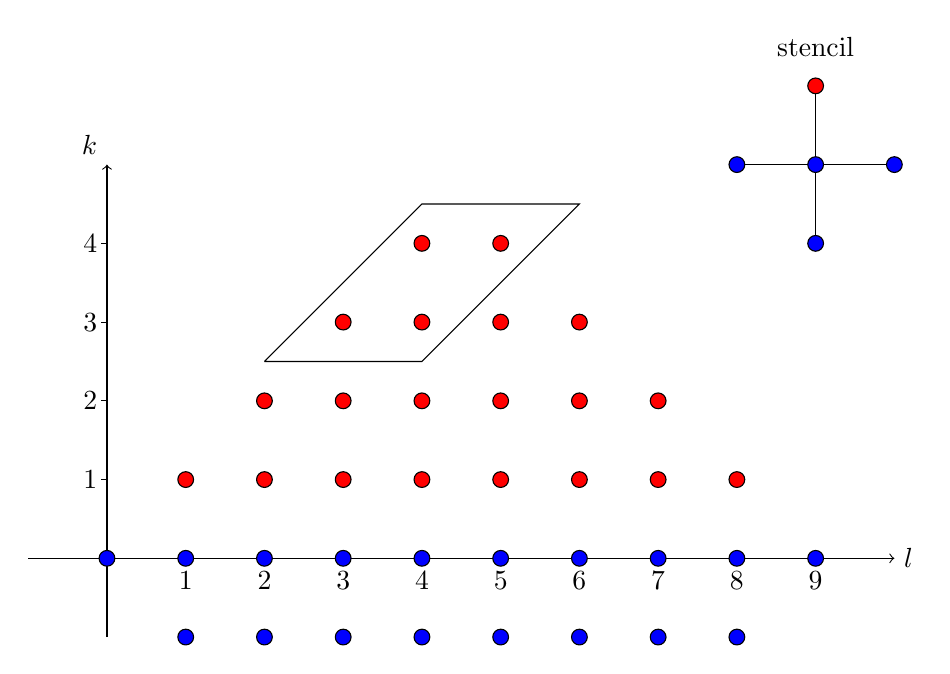
\begin{tikzpicture}[scale=1.0]
\draw[->] (0, -1) -- (0, 5);
\node[above left] at (0, 5) {$k$};
\draw[->] (-1, 0) -- (10, 0);
\node[right] at (10, 0) {$l$};
\foreach \x in {1, 2, ..., 8}
    \draw[fill=blue] (\x, -1) circle(0.10cm);
\foreach \x in {0, 1, ..., 9}
    \draw[fill=blue] (\x, 0) circle(0.10cm);
\foreach \x in {1, 2, ..., 8}
    \draw[fill=red] (\x, 1) circle(0.10cm);
\foreach \x in {2, 3, ..., 7}
    \draw[fill=red] (\x, 2) circle(0.10cm);
\foreach \x in {3, 4, 5, 6}
    \draw[fill=red] (\x, 3) circle(0.10cm);
\foreach \x in {4, 5}
    \draw[fill=red] (\x, 4) circle(0.10cm);
\foreach \y in {1, 2, 3, 4}
    {
    \draw[thin] (-0.075, \y) -- (0, \y);
    \node[left] at (0.0, \y) {$\y$};
    }
\foreach \x in {1, 2, 3, ..., 9}
    \node[below] at (\x, -0.04) {$\x$};
\draw[-] (9, 4) -- (9, 6);
\draw[-] (8, 5) -- (10, 5);
\draw[fill=blue] (8, 5) circle(0.10cm);
\draw[fill=blue] (9, 5) circle(0.10cm);
\draw[fill=blue] (10, 5) circle(0.10cm);
\draw[fill=blue] (9, 4) circle(0.10cm);
\draw[fill=red]  (9, 6) circle(0.10cm);
\node at (9, 6.5) {stencil};
\draw[-] (2.0, 2.5) -- (4.0, 4.5) -- (6.0, 4.5) 
      -- (4.0, 2.5) -- (2.0, 2.5);
\end{tikzpicture}
\end{center}
\end{figure}

The algorithm requires that we know the values of the integrals
\[
\mu_k=\int p_k(x)\,d\mu(x)\quad\text{for $0\le k\le 2n-1$,}
\]
and is summarised in the following theorem.

\begin{theorem}
The coefficients $\alpha_k$~and $\beta_k$ in the three-term 
recurrence relation~\eqref{eq: 3 term q} can be computed 
for $0\le k\le n-1$ by putting
\[
\begin{aligned}
\sigma_{l,-1}&=0&\text{for $1\le l\le 2n-2$},\\
\sigma_{l,0}&=\mu_l&\text{for $0\le l\le2n-1$},\\
\alpha_0&=a_0+\frac{\mu_1}{\mu_0},\\
\beta_0&=\mu_0,
\end{aligned} 
\]
and, for $k=1$, $2$, \dots, $n-1$ and $k\le l\le2n-k-1$, 
\[
\begin{aligned}
\sigma_{lk}&=\sigma_{l+1,k-1}+(a_l-\alpha_{k-1})\sigma_{l,k-1}
		+b_l\sigma_{l-1,k-1}-\beta_{k-1}\sigma_{l,k-2},\\
\alpha_k&=a_k+\frac{\sigma_{k+1,k}}{\sigma_{kk}}
	-\frac{\sigma_{k,k-1}}{\sigma_{k-1,k-1}},\\
\beta_k&=\frac{\sigma_{kk}}{\sigma_{k-1,k-1}}.
\end{aligned}
\]
\end{theorem}
\begin{proof}
It is easily verified that the integrals
\[
\sigma_{lk}=\int p_l(x)q_k(x)\,d\mu(x)
\]
satisfy the initial conditions $\sigma_{l,-1}=0$~and 
$\sigma_{l,0}=\mu_l$.  In addition, $\sigma_{lk}=0$ if $k>l$. 
For $1\le k\le l$,
\begin{align*}
\sigma_{lk}&=\int p_l(x)\bigl[
	(x-\alpha_{k-1})q_{k-1}(x)-\beta_{k-1}q_{k-2}(x)\bigr]\,d\mu(x)\\
	&=\int(x-a_l+a_l-\alpha_{k-1})p_l(x)q_{k-1}(x)\,d\mu(x)
		-\beta_{k-1}\sigma_{l,k-2}\\
	&=\int\bigl[(x-a_l)p_l(x)-b_lp_{l-1}(x)\bigr]
		q_{k-1}(x)\,d\mu(x)\\
	&\qquad{}+(a_l-\alpha_{k-1})\sigma_{l,k-1}
		+b_l\sigma_{l-1,k-1}-\beta_{k-1}\sigma_{l,k-2}
\end{align*}
so
\[
\sigma_{lk}=\sigma_{l+1,k-1}+(a_l-\alpha_{k-1})\sigma_{l,k-1}
		+b_l\sigma_{l-1,k-1}-\beta_{k-1}\sigma_{l,k-2}.
\]

Recall that
\[
\alpha_k=\int xq_k(x)^2\,\mu(x)\bigg/\int q_k(x)^2\,d\mu(x)
\]
and
\[
\beta_k=\int q_k(x)^2\,\mu(x)\bigg/\int q_{k-1}(x)^2\,d\mu(x).
\]
Since $q_k(x)-p_k(x)$ has degree at most~$k-1$, the orthogonality 
property of the $q_k$ implies that
\begin{align*}
\int q_k(x)^2\,d\mu(x)&=\int p_k(x)q_k(x)\,d\mu(x)
	+\int\bigl[q_k(x)-p_k(x)\bigr]q_k(x)\,d\mu(x)\\
	&=\sigma_{kk}+0,
\end{align*}
so
\[
\beta_k=\frac{\sigma_{kk}}{\sigma_{k-1,k-1}}\quad\text{for $k\ge1$,}
	\qquad\text{with $\beta_0=\mu_0$.}
\]
Similarly,
\[
\int x q_k(x)^2\,d\mu(x)
	=\int x\bigl[q_k(x)-p_k(x)\bigr]q_k(x)\,d\mu(x)
	+\int xp_k(x)q_k(x)\,d\mu(x),
\]
with
\begin{align*}
\int x&\bigl[q_k(x)-p_k(x)\bigr]q_k(x)\,d\mu(x)
	=\int\bigl[q_k(x)-p_k(x)\bigr](x-\alpha_k)q_k(x)\,d\mu(x)\\
	&\qquad\qquad\qquad\qquad\qquad\qquad{}+\alpha_k\int 
		\bigl[q_k(x)-p_k(x)\bigr]q_k(x)\,d\mu(x)\\
	&=\int\bigl[q_k(x)-p_k(x)\bigr]
	\bigl[q_{k+1}(x)+\beta_k q_{k-1}(x)\bigr] 
		\,d\mu(x)+\alpha_k\times0\\
	&=-\beta_k\sigma_{k,k-1}=-\frac{\sigma_{kk}}{\sigma_{k-1,k-1}}
	\,\sigma_{k,k-1}
\end{align*}
and
\begin{align*}
\int xp_k(x)q_k(x)\,d\mu(x)&=\int\bigl[
	(x-a_k)p_k(x)-b_kp_{k-1}(x)\bigr]q_k(x)\,d\mu(x)\\
	&\qquad{}+\int\bigl[
		a_kp_k(x)+b_kp_{k-1}(x)\bigr]q_k(x)\,d\mu(x)\\
	&=\int p_{k+1}(x)q_k(x)\,d\mu(x)+a_k\int p_k(x)q_k(x)\,d\mu(x)\\
	&=\sigma_{k+1,k}+a_k\sigma_{kk};
\end{align*}
thus,
\[
\alpha_k=a_k+\frac{\sigma_{k+1,k}}{\sigma_{kk}}
	-\frac{\sigma_{k,k-1}}{\sigma_{k-1,k-1}}
	\quad\text{for $k\ge1$,}
\]
with
\[
\alpha_0=\frac{\sigma_{10}+a_0\sigma_{00}-\beta_0\sigma_{0,-1}}%
{\sigma_{00}}=a_0+\frac{\sigma_{10}}{\sigma_{00}}
	=a_0+\frac{\mu_1}{\mu_0}.
\]
\end{proof}
%%%%%%%%%%%%%%%%%%%%%%%%%%%%%%%%%%%%%%%%%%%%%%%%%%%%%%%%%%%%%%%%%%%%%
\section{A log weight}
We now consider the example
\[
d\mu(x)=x^\rho\log x^{-1}\,dx\quad\text{for $0<x<1$,}
\]
with $\rho>-1$.  As our second family of orthogonal polynomials we 
use the shifted Legendre polynomials,
\[
p_k(x)=P_k(2x-1);
\]
thus
\[
\mu_k=\int_0^1 P_k(2x-1)x^\rho\log x^{-1}\,dx.
\]
Following \cite{Gautschi1979}, we make the substitution $y=2x-1$
and obtain
\[
\mu_k=\frac{\log 2}{2^{\rho+1}}\int_{-1}^1 P_k(y)(y+1)^\rho\,dy
	-\frac{1}{2^{\rho+1}}\int_{-1}^1 
		P_k(y)(y+1)^\rho\log(y+1)\,dy
\]
It is known that
\[
\int_{-1}^1 P_k(y)(y+1)^\rho\,dy
	=\frac{2^{\rho+1}\Gamma(\rho+1)^2}%
{\Gamma(\rho+k+2)\Gamma(\rho+1-k)},
\]
and by logarithmic differentiation of this identity with respect 
to~$\rho$, we find that
\begin{multline*}
\int_{-1}^1 P_k(y)(y+1)^\rho\log(y+1)\,dy
	=\frac{2^{\rho+1}\Gamma(\rho+1)^2}%
{\Gamma(\rho+k+2)\Gamma(\rho+1-k)}\\
	\times\bigl[\log2+2\psi(\rho+1)-\psi(\rho+k+2)-\psi(\rho+1-k)
	\bigr],
\end{multline*}
where $\psi(x)=\Gamma'(x)/\Gamma(x)$ denotes the digamma function.
Thus,
\[
\mu_k=\frac{\Gamma(\rho+1)^2}{\Gamma(\rho+k+2)\Gamma(\rho+1-k)}
	\bigl[\psi(\rho+k+2)+\psi(\rho+1-k)-2\psi(\rho+1)\bigr].
\]
Using the reflection formulae
\[
\Gamma(1-z)\Gamma(z)=\frac{\pi}{\sin\pi z}
\quad\text{and}\quad
\psi(1-z)=\psi(z)+\pi\cot\pi z,
\]
we find that
\[
\lim_{z\to m}\frac{\psi(-z)}{\Gamma(-z)}=(-1)^{m+1}m!
\quad\text{for $m\in\{0,1,2,\dots\}$.}
\]




that if $\rho=m$ is an integer
It is known~
\[
\mu_r=(-1)^{r-m}\,\frac{(m!)^2(r-m-1)!}{(r+m+1)!}
\]







%%%%%%%%%%%%%%%%%%%%%%%%%%%%%%%%%%%%%%%%%%%%%%%%%%%%%%%%%%%%%%%%%%%%%
\bibliographystyle{plain}
\bibliography{notes_refs}
%%%%%%%%%%%%%%%%%%%%%%%%%%%%%%%%%%%%%%%%%%%%%%%%%%%%%%%%%%%%%%%%%%%%%
\end{document}
\endinput
